\documentclass[twocolumn]{article}
\usepackage[portrait,margin=2cm]{geometry}

\title{AI 1103 Assignment-1}
\author{Shantanu Pandey\\ CS20BTECH11046}
\date{}
\usepackage{amsmath}
\usepackage{amssymb}
\usepackage{amsfonts}
\usepackage{nopageno}
% \usepackage[margin=1in]{geometry}
\usepackage{graphicx}
\usepackage{float}
\usepackage{multicol}
\usepackage{hyperref}
\setlength{\columnsep}{0.5cm}
\setlength{\parindent}{0em}
\usepackage{color}
\usepackage{comment}
\setlength{\columnseprule}{1pt}
\def\columnseprulecolor{\color{black}}


\providecommand{\mbf}{\mathbf}
\providecommand{\pr}[1]{\ensuremath{\Pr\left(#1\right)}}
\providecommand{\qfunc}[1]{\ensuremath{Q\left(#1\right)}}
\providecommand{\sbrak}[1]{\ensuremath{{}\left[#1\right]}}
\providecommand{\lsbrak}[1]{\ensuremath{{}\left[#1\right.}}
\providecommand{\rsbrak}[1]{\ensuremath{{}\left.#1\right]}}
\providecommand{\brak}[1]{\ensuremath{\left(#1\right)}}
\providecommand{\lbrak}[1]{\ensuremath{\left(#1\right.}}
\providecommand{\rbrak}[1]{\ensuremath{\left.#1\right)}}
\providecommand{\cbrak}[1]{\ensuremath{\left\{#1\right\}}}
\providecommand{\lcbrak}[1]{\ensuremath{\left\{#1\right.}}
\providecommand{\rcbrak}[1]{\ensuremath{\left.#1\right\}}}


\newcommand*{\permcomb}[4][0mu]{{{}^{#3}\mkern#1#2_{#4}}}
\newcommand*{\perm}[1][-3mu]{\permcomb[#1]{P}}
\newcommand*{\comb}[1][-1mu]{\permcomb[#1]{C}}

\begin{document}
\maketitle
\noindent
Download all python codes from here

% \begin{multicols*}{2}
\noindent
\fbox{%
    \parbox{0.45\textwidth}{%
        \url{ https://github.com/Shantanu467/AI1103/blob/main/Assignemt_1/codes/Assignemt1.py }
    }%
    }
    
\vspace{0.3cm}
and latex-tikz codes from  

\vspace{0.3cm}  
    
\fbox{%
    \parbox{0.45\textwidth}{%
        \url{https://github.com/Shantanu467/AI1103/blob/main/Assignemt_1/codes/Assignmet-1.tex}
    }%
    }
   
\vspace{0.5cm}
\textbf{QUESTION-4.7}
\vspace{0.5cm} 

A bag consists of 10 balls each marked with
one of the digits 0 to 9. If four balls are drawn
successively with replacement from the bag,
what is the probability that none is marked
with the digit 0?

\vspace{0.5cm}
\textbf{SOLUTION}
\vspace{0.5cm} 



Let $X$ be number marked on ball drawn.
Since the balls are drawn with replacement, the trials are Bernoulli trials.
\\
So $X$ has Binomial Distribution 
\begin{equation}
    \pr {X=k}=\comb{n}{k} \times q^{n-k} \times p^{k} 
\end{equation} 

Here,
\begin{align}
& n = \text {number of times we pick the ball}  \\
& p= \text{Probability of getting ball marked as 0} \\
& q=1-p
\end{align}

\begin{table}[h!]
\centering

\begin{tabular}{|c|c|c|c|c|}
\hline
\textbf{Variables} & $n$ & $p$    & $q$    & $k$          \\ \hline
\textbf{Values}    & 4 & 1/10 & 9/10 & 0 \\ \hline
\end{tabular}
\caption{Variables and their values}
\label{table:1}
\end{table}

Now,

\begin{align}
\pr{X=0} &= \comb{4}{0} \times \brak{\frac{9}{10}}^{(4-0)} \times \brak{\frac{1}{10}}^{0} \\
&=\frac{4!}{(4-0)! 0!} \times 1 \times \brak{\frac{9}{10}}^{4} \\
&=\brak { \frac{9}{10} } ^{4} \\
&= 0.6561
\end{align}
Therefore, The probability that none of ball is marked with $0$ is \textbf{0.6561}

 \vspace{1cm}


\begin{figure} [h!]
    \centering
    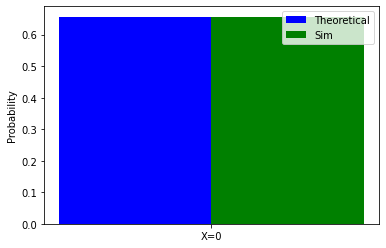
\includegraphics[scale=0.65]{Assignment1.png}
    \caption{The close relation between
Theoretical and simulated results.}
    \label{fig:my_label}
\end{figure}
 % \end{multicols*}


\end{document}
